\documentclass[11pt]{article}
\usepackage[utf8]{inputenc}
\usepackage[T1]{fontenc}
\usepackage{graphicx}
\usepackage[export]{adjustbox}
\graphicspath{ {./images/} }
\usepackage{amsmath}
\usepackage{amsfonts}
\usepackage{amssymb}
\usepackage[version=4]{mhchem}
\usepackage{stmaryrd}
\usepackage{hyperref}
\hypersetup{colorlinks=true, linkcolor=blue, filecolor=magenta, urlcolor=cyan,}
\urlstyle{same}

\begin{document}
Four Core Dimensions of Managed Futures Investment Strategies

Managed futures strategies can be divided across four core dimensions: data sources, implementation style, strategy focus, and time horizon. The next exhibit presents a diagram of managed futures strategies.

\begin{center}
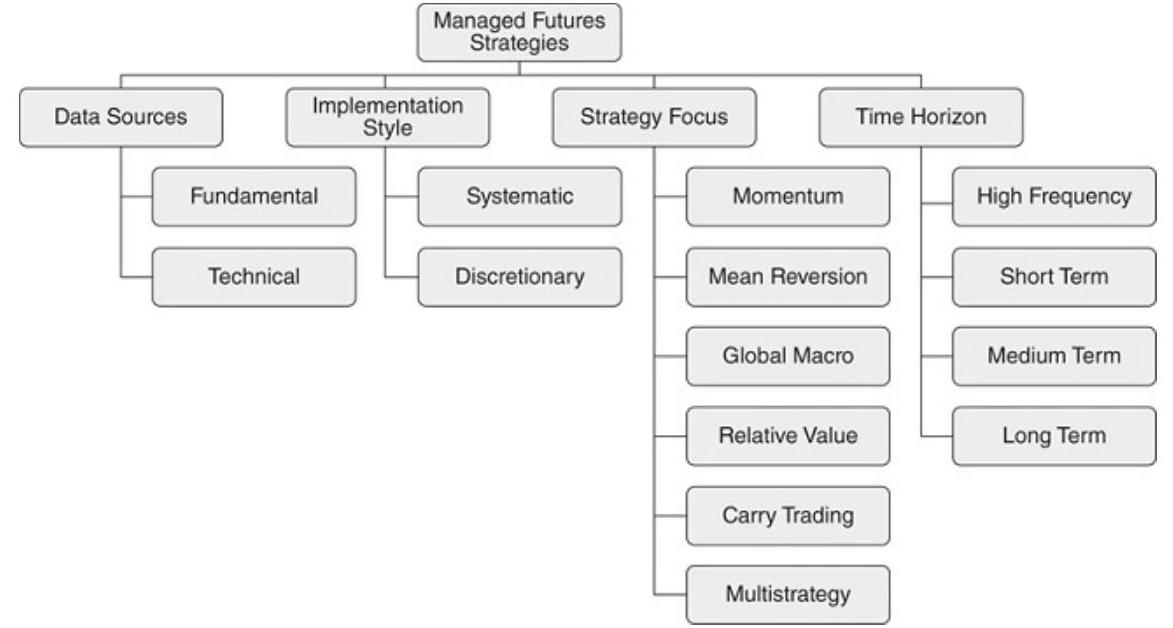
\includegraphics[max width=\textwidth]{2024_04_09_bb15184d6b10431fa36bg-2}
\end{center}

Dimensions of Managed Futures Strategies

\section*{Data Sources as a Core Managed Futures Dimension}
Managed futures strategies are often denoted as either fundamental or technical. Fundamental strategies rely on such data as economic forecasts, supply and demand estimates, and crop rotation schedules, whereas technical strategies typically analyze historical information such as price and volume. Strategies are also categorized into implementation styles of either systematic or discretionary. Systematic (or quantitative) strategies follow a series of rules to determine entry and exit conditions, position scaling, and position sizes. These strategies rely mostly on the outputs of quantitative models rather than the manager's direct intervention. In terms of turnover, systematic strategies may vary greatly in terms of trade horizon, where trades are held from seconds to months. Over time, systematic strategies have grown in complexity, designed by quant teams that develop the models and automate trading execution. Systematic trading programs also require extensive data capabilities, trading support, and technical support. Systematic implementation is often used in the futures space, given the complexities of futures trading. Trading systems allow a CTA to allocate across many futures markets, maintain collateral, and control and monitor a large number of positions.

\section*{Implementation Style as a Core Managed Futures Dimension}
Systematic programs are typically more broadly diversified than discretionary traders, both in the number of markets analyzed and in the types of strategies employed. Discretionary managed futures strategies are implemented at the discretion of a CTA manager. These strategies seek to participate opportunistically in market-driven price actions, with the final trading decision being made at the discretion of the fund manager. Since many discretionary managers also use quant models to determine positions, the line between purely discretionary and systematic can sometimes be blurred. ${ }^{1}$ Peter Park, Oguz Tanrikulu, and Guodong Wang, "Systematic Global Macro: Performance, Risk and Correlation Characteristics" (January 2009). Working paper. Available at

\href{https://www.trendfollowing.com/pdfs/tropin.pdf}{https://www.trendfollowing.com/pdfs/tropin.pdf}.

\section*{Strategy Focus as a Core Managed Futures Dimension}
Given the range of possible asset classes in futures markets, the range of strategies is relatively broad. Common strategies in the space, discussed in previous sectors, include momentum, mean reversion, and relative value. Other strategies include carry trading, multistrategy, and global macro.

Global macro managed futures strategies use fundamental information to determine long and short allocations across the global range of futures markets. Global macro futures strategies will take positions in foreign exchange, commodities, domestic and international equity, and fixed-income markets based on fundamental analysis. A global macro strategy can develop economic models that attempt to explain how the global economy will react to various changes in economic regimes. For example, if the U.S. dollar appreciates, this improves the purchasing power of the U.S. dollar while decreasing the attractiveness of U.S. exports. A global macro manager can construct an economic model that attempts to predict both U.S. dollar exchange rates and the economic impact on commodities, global stock markets, and short- and long-term rates. Another macro strategy may use fundamental inputs and data to gauge the change in the demand for oil. If a global macro manager's model predicts an increase in demand, the manager will go long oil; if demand is predicted to decrease, the manager will short oil. Global macro managers and trend-following strategies use different inputs to determine where global trends will occur. Because of this, the performance of discretionary versus systematic managed futures can vary. Another key difference between the two is that a fundamentally based strategy is more likely to enter a global trend earlier than a trendfollowing strategy will. This is because trend-following strategies need to measure momentum in prices to begin a position. Although global macro strategies often get in earlier, the market may not agree with the fundamentals for long periods of time, causing difficulty for global macro strategies.

Mean-reversion and countertrend strategies focus on prices reverting to the mean in the short term. Mean-reversion strategies are typically implemented in days to weeks, whereas trend following is often implemented in months. A strategy is considered contrarian if it trades against the prevalent trend. Mean-reversion strategies often take contrarian positions. A contrarian strategy would have the opposite sign of a trend-following strategy. Carry strategies are designed to take advantage of differences in the carry of various commodities. In general, the carry of an asset is the return obtained from holding it (if positive) or the cost of holding it (if negative). For instance, commodities are usually negative carry assets, as they incur storage costs and may suffer from depreciation; however, appropriately hedged commodities can be positive carry assets if the futures market is willing to pay a sufficient premium for future delivery. Carry trades involve long positions in fixed-\\
income investments of high interest rate countries and short positions in fixed-income investments of low interest rate countries. Multistrategy CTAs combine a variety of strategy focuses to provide a diversified set of potential return sources and risk-reward profiles.

\section*{Time Horizon as a Core Managed Futures Dimension}
The final aspect that differentiates managed futures strategies is time horizon. Time horizons can range from high frequency to long term. Trading speed is often measured by the average holding period for each trade. High-frequency trading is reserved for a special group of strategies that do not attempt to benefit from trends in prices and traditionally have not been classified as managed futures strategies. Short-term CTA trading strategies are often classified as intraday to one month, with an average holding period of around 10 days or less. Medium term can be one month to six months. Long term can be greater than six months. Mean reversion and countertrend tend to be shorter term, whereas trend following is often medium to long term. It is very common for systematic funds to combine a large range of approaches, from short term to long term.

A core issue in dynamic futures trading strategies is transaction costs, trading capacity, and slippage. Transaction costs are incurred on a per trade basis. As a result, transaction costs are very important for short-term strategies that may require frequent transactions. Medium- to long-term strategies focus on longer-term effects. As a result, they do not adjust their positions as quickly or as often as do shorter-term programs. Trading capacity is important for strategies that take large positions relative to open interest. If a strategy requires large short-term changes in positions, the strategy may move the market against the strategy. Since CTAs manage accounts on behalf of clients, they often trade multiple accounts simultaneously. This could lead to slippage. Slippage occurs when actual performance deviates or "slips away" from the expected trading results using the computer's signal.


\end{document}